%%%%%%%%%%%%%%%%%%%%%%%%%%%%%%%%%%%%%%%%%
% Short Sectioned Assignment
% LaTeX Template
% Version 1.0 (5/5/12)
%
% This template has been downloaded from:
% http://www.LaTeXTemplates.com
%
% Original author:
% Frits Wenneker (http://www.howtotex.com)
%
% License:
% CC BY-NC-SA 3.0 (http://creativecommons.org/licenses/by-nc-sa/3.0/)
%
%%%%%%%%%%%%%%%%%%%%%%%%%%%%%%%%%%%%%%%%%

%----------------------------------------------------------------------------------------
%	PACKAGES AND OTHER DOCUMENT CONFIGURATIONS
%----------------------------------------------------------------------------------------

\documentclass[paper=a4, fontsize=11pt]{scrartcl} % A4 paper and 11pt font size
\usepackage[margin=0.7in]{geometry}
\usepackage[T1]{fontenc} % Use 8-bit encoding that has 256 glyphs
\usepackage{fourier} % Use the Adobe Utopia font for the document - comment this line to return to the LaTeX default
\usepackage[english]{babel} % English language/hyphenation
\usepackage{amsmath,amsfonts,amsthm} % Math packages

\usepackage{lipsum} % Used for inserting dummy 'Lorem ipsum' text into the template

\usepackage{sectsty} % Allows customizing section commands
\allsectionsfont{\bfseries\sffamily\scshape} % Make all sections centered, the default font and small caps

\usepackage{fancyhdr} % Custom headers and footers
\pagestyle{fancyplain} % Makes all pages in the document conform to the custom headers and footers
\fancyhead{} % No page header - if you want one, create it in the same way as the footers below
\fancyfoot[L]{} % Empty left footer
\fancyfoot[C]{} % Empty center footer
\fancyfoot[R]{\thepage} % Page numbering for right footer
\renewcommand{\headrulewidth}{0pt} % Remove header underlines
\renewcommand{\footrulewidth}{0pt} % Remove footer underlines
\setlength{\headheight}{13.6pt} % Customize the height of the header

\numberwithin{equation}{section} % Number equations within sections (i.e. 1.1, 1.2, 2.1, 2.2 instead of 1, 2, 3, 4)
\numberwithin{figure}{section} % Number figures within sections (i.e. 1.1, 1.2, 2.1, 2.2 instead of 1, 2, 3, 4)
\numberwithin{table}{section} % Number tables within sections (i.e. 1.1, 1.2, 2.1, 2.2 instead of 1, 2, 3, 4)

\setlength\parindent{0pt} % Removes all indentation from paragraphs - comment this line for an assignment with lots of text

\usepackage[english]{babel}
\usepackage{graphicx}
\usepackage{listings}
\usepackage{amsmath}

%----------------------------------------------------------------------------------------
%	TITLE SECTION
%----------------------------------------------------------------------------------------

\newcommand{\horrule}[1]{\rule{\linewidth}{#1}} % Create horizontal rule command with 1 argument of height

\title{	
\normalfont \normalsize 
\textsc{University of Southern California, Computer Science} \\ [25pt] % Your university, school and/or department name(s)
\horrule{0.5pt} \\[0.4cm] % Thin top horizontal rule
\huge Machine Learning: HomeWork 4 \\ % The assignment title
\horrule{2pt} \\[0.5cm] % Thick bottom horizontal rule
}

\author{Rohit Kondekar\\
740-581-9473} % Your name

\date{\normalsize\today} % Today's date or a custom date
\allowdisplaybreaks
\begin{document}

\maketitle % Print the title


%----------------------------------------------------------------------------------------
%	PROBLEM 1
%----------------------------------------------------------------------------------------
\section{Question: Boosting}
\subsection{Gradient Calculation}

\begin{align*} 
\textbf{Least Squared Loss:}~~~  L(y_{i},\hat{y}_i) &= (y_{i} - \hat{y}_i)^{2}\\
\textbf{Gradient of Loss:} ~~~ g_{i} &= \dfrac{\partial L(y_{i},\hat{y}_i) }{\partial \hat{y}_i}\\
 g_{i} &= -2(y_{i} - \hat{y}_i)
\end{align*}

\subsection{Weak Learner Selection}
\begin{align*}
\gamma^{*} &= \texttt{argmin}_{\gamma \in R} \sum_{i=1}^{n}(-g_{i}- \gamma h(x_{i}))^{2}\\
&= \texttt{argmin}_{\gamma \in R} \sum_{i=1}^{n}(2(y_{i} - \hat{y}_i)- \gamma h(x_{i}))^{2}
\end{align*}
Differentiating w.r.t $\gamma$ and equating to zero
\begin{align*}
\sum_{i=1}^{n} -2h(x_{i}) [2(y_{i} - \hat{y}_i)- \gamma h(x_{i})] &= 0\\
\sum_{i=1}^{n} [-4h(x_{i})(y_{i} - \hat{y}_i) + 2\gamma h(x_{i})^{2}] &=0\\
2\gamma \sum_{i=1}^{n} h(x_{i})^{2} &= 4\sum_{i=1}^{n} h(x_{i})(y_{i} - \hat{y}_i)\\
\gamma &=  \dfrac{2\sum_{i=1}^{n} h(x_{i})(y_{i} - \hat{y}_i)}{\sum_{i=1}^{n} h(x_{i})^{2}}
\end{align*}

\subsection{Step Size Selection}
\begin{align*}
\alpha^{*} &= \texttt{argmin}_{\alpha \in R}  \sum_{i=1}^{n} (y_{i} - (\hat{y}_{i} + \alpha h^{*}(x_{i})))^{2}
\end{align*}

Differentiating w.r.t $\alpha$ and equating to zero

\begin{align*}
\sum_{i=1}^{n} -2h^{*}(x_{i})(y_{i} - \hat{y}_{i} - \alpha h^{*}(x_{i})) &=0\\
\sum_{i=1}^{n} [-2h^{*}(x_{i})y_{i} + 2h^{*}(x_{i})\hat{y}_{i} + 2\alpha h^{*}(x_{i})^{2}] &=0 \\
2\sum_{i=1}^{n} \alpha h^{*}(x_{i})^{2} &= 2\sum_{i=1}^{n}[h^{*}(x_{i}) (y_{i} - \hat{y}_{i})]\\
\alpha &= \dfrac{\sum_{i=1}^{n}h^{*}(x_{i}) (y_{i} - \hat{y}_{i})}{\sum_{i=1}^{n} h^{*}(x_{i})^{2}}
\end{align*}



\section{Question: Neural Network}
\subsection{}
As the question says the network has logistic output and linear activation function in hidden layer, the prediction function can be written as, where w is weights of second layer and v are weights of first layer:

\begin{align*}
y &= \sigma (\sum_{k}w_{k} \times (\sum_{i}v_{ki}x_{i}))\\
&= \dfrac{1}{1 + \exp(-\sum_{k}w_{k} \times (\sum_{i}v_{ki}x_{i}))}\\
&= \dfrac{1}{1 + \exp(-\sum_{k}\sum_{i}w_{k}v_{ki}x_{i})}\\
& = \dfrac{1}{1 + \exp(-\sum_{i}w_{i}^{'}x_{i})}~~~~
\textsf{ Where $w_{i}^{'} = \sum_{k}w_{k}v_{ki}$}
\end{align*}
This shows thats its similar to logistic regression, with different weights combination. Even if there are multiple hidden layers, the equation would be in similar format.

\subsection{}
\begin{figure}[h!]
  \centering
    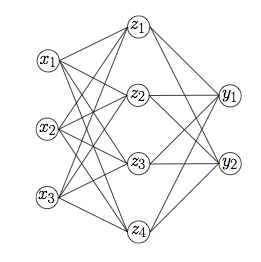
\includegraphics[width=0.3\textwidth]{../figures/neuralNetwork.png}
  \caption{Neural Network}
\end{figure}

\begin{align*}
L(y,\hat{y}) &= \dfrac{1}{2} \sum_{j=1}^{2} (y_{j} - \hat{y_{j}})^{2}\\
\end{align*}

First finding gradient for $v_{jk}$:
\begin{align*}
\dfrac{\partial L}{\partial v_{jk}} &= \dfrac{\partial L}{\partial b_{j}} \dfrac{\partial b_{j}}{\partial v_{jk}} ~~~ \textsl{where $b_{j} = \hat{y}_{j} = \sum_{k}v_{jk}z_{k}$}\\
\dfrac{\partial L}{\partial v_{jk}} &= -(y_{j} - \hat{y}_{j})z_{k}\\
\end{align*}

Now finding gradient for $w_{ki}$:

\begin{align*}
\dfrac{\partial L}{\partial w_{ki}} &= \dfrac{\partial L}{\partial a_{k}} \dfrac{\partial a_{k}}{\partial w_{ki}} ~~~
\textsl{where $a_{k} = \sum_{k}w_{ki}x_{i}$}\\
&= \dfrac{\partial L}{\partial a_{k}} x_{i}\\
&= \sum_{j} \dfrac{\partial L}{\partial b_{j}} \dfrac{\partial b_{j}}{\partial a_{k}} x_{i}\\
&= \sum_{j} (y_{j}-\hat{y}_{j})\dfrac{\partial (v_{jk}tanh(a_{k}))}{\partial a_{k}} x_{i}\\
&= \sum_{j}^{2} (y_{j}-\hat{y}_{j}) v_{jk} (1-tanh^{2}(\sum_{i}^{3}w_{ki}x_{i})) x_{i}
\end{align*}



\section{Question: Clustering}
\subsection{}
\begin{align*}
D &= \sum_{n=1}^{N}\sum_{k=1}^{K}r_{nk} ||x_{n} - \mu_{k}||_{2}^{2}\\
&= \sum_{n=1}^{N}\sum_{k=1}^{K} r_{nk} (x_{n} - \mu_{k})^{T}(x_{n} - \mu_{k})\\
&= \sum_{n=1}^{N}\sum_{k=1}^{K} r_{nk} (x_{n}^{T}x_{n} - x_{n}^{T}\mu_{k} - \mu_{k}^{T}x_{n} + \mu_{k}^{T}\mu_{k})\\
\dfrac{\partial D}{\partial \mu_{k}} &=  \sum_{n=1}^{N} r_{nk} (2\mu_{k} - 2x_{n}) = 0\\\
\sum_{n=1}^{N} r_{nk}\mu_{k} &= \sum_{n=1}^{N}r_{nk}x_{n}\\
\mu_{k} &= \dfrac{\sum_{n=1}^{N}r_{nk}x_{n}}{\sum_{n=1}^{N} r_{nk}}
\end{align*}

This shows that to minimize this loss/cost function, $\mu$ has to be the mean of the respective clusters.

\subsection{}
\begin{align*}
D &= \sum_{n=1}^{N}\sum_{k=1}^{K}r_{nk} ||x_{n} - \mu_{k}||_{1}\\
\end{align*}

Intutively, we can see here that the cost function is bascically sum of the difference between $\mu$ and each data point.\\
If we sort the array and choose the last and first point (i.e. the points which are farthest), the point which is closest to all other points, will the point which lies in center. i.e. equidistant from all the points.\\\\
So if n is odd the the point will be at $\dfrac{i+j}{2}$th location. else if even it would be the the average of two middle elements.\\\\

\textbf{It can be shown as:}\\
If we have an even number of points, there will be two medians. A point between the two medians will have n/2 points to the left and n/2 points to the right, and a total sum-of-distances to those points of S.\\\\
If we move it one point to the left, S will go up by n/2 (since we're moving away from the right-most points) and down by n/2 (since we're moving towards the left-most points), so overall S remains the same. This holds true until we hit the left-most median point. When we move one left of the left-most median point, we now have (n/2 + 1) points to the right, and (n/2 - 1) points to the left, so S goes up by two. Continuing to the left will only increase S further.\\\\
By the same logic, all points to the right of the right-most median also have a higher S.\\\\
If we have an odd number of points, there is only one median. Using the same logic as above, we can show that it has the lowest value of S.\\\\
\textbf{Mathematically:}\\
\begin{align*}
\dfrac{\partial D}{\partial \mu_{k}} &= \sum_{n=1}^{N}\sum_{k=1}^{K}r_{nk} sign(x_{n} - \mu_{k}) = 0
\end{align*}

Calculating for a perticular cluster of size m:

\begin{align*}
\sum_{m=1}^{M} sign(x_{m} - \mu_{k}) &= 0\\
sign(x_{m} - \mu_{k}) &= +1 ~~~\textsl{if}~~ x_{m} - \mu_{k}>0\\
&= -1 ~~~\textsl{if}~~ x_{m} - \mu_{k}<0\\
\end{align*}

Therefore: $\Psi(x_{n}|x_{n} - \mu_{k}>0) - \Psi(x_{n}|x_{n} - \mu_{k}<0) = 0$ where $\Psi$ denotes number of elements.\\\\
This becomes zero pricisely at median.

\section{Question: Mixture Models}
\subsection{}
$X_{i} \sim \exp(\lambda)$\\
$Y_{i} = min(X_{i},c_{i})$\\

Therefore, in this problem the observed variables are $Y_{i}=X_{i} : 0<i<=r$ \\
The hidden variables are $Y_{i}=X_{i} : r+1<= i <=n$ \\
And the parameter is $\lambda$\\


\begin{align*}
\textbf{Likelihood:}~~~ L(\lambda) &= \prod_{i=1}^{n} \lambda e^{-\lambda x_{i}}\\
&= \lambda^{n} e^{-\lambda \sum_{i}^{n}X_{i}}\\
\textbf{Log Likelihood:}~~~ l(\lambda) &= n\log(\lambda) - \lambda \sum_{i=1}^{n}X_{i}\\
&= n\log(\lambda) - \lambda [\sum_{i=1}^{r}X_{i} + \sum_{j=r+1}^{n}X_{j}]
\end{align*}

\subsection{}
E Step is where we take the Expectation of Log Likelihood. Assume $Z = X_{r+1}.....X_{n}$ i.e. the unoberved data.
\begin{align*}
E_{Z|Y}[l(\lambda)] &= E_{Z|Y}[n\log(\lambda) - \lambda [\sum_{i=1}^{r}X_{i} + \sum_{j=r+1}^{n}X_{j}]]\\
&= n\log(\lambda) - \lambda \sum_{i=1}^{r}X_{i} - E_{Z|Y}[ \sum_{j=r+1}^{n}X_{j}]\\
&= n\log(\lambda) - \lambda \sum_{i=1}^{r}X_{i} - \sum_{j=r+1}^{n}E_{Z|Y}[X_{j}]\\
&= n\log(\lambda) - \lambda \sum_{i=1}^{r}X_{i} - \sum_{j=r+1}^{n}E_{X_{j}|Y_{j}}[X_{j}]\\
&= n\log(\lambda) - \lambda \sum_{i=1}^{r}X_{i} - \sum_{j=r+1}^{n}E_{X_{j}|Y_{j}}[X_{j}>c_{j}]\\
&= n\log(\lambda) - \lambda \sum_{i=1}^{r}X_{i} - \sum_{j=r+1}^{n}(c_{j}+\dfrac{1}{\lambda^{k}})~~~\textbf{Because of memoryless property of exponential distribution.}\\
Q(\lambda,\lambda^{k}) = E_{Z|Y}[l(\lambda)] &= n\log(\lambda) - \lambda \sum_{i=1}^{r}X_{i} - \sum_{j=r+1}^{n}(c_{j}+\dfrac{1}{\lambda^{k}})
\end{align*}

\subsection{}

In M-step we will maximize the $Q(\lambda,\lambda^{k})$ w.r.t $\lambda$ i.e.
\begin{align*}
\lambda^{k+1} &= \textsl{argmax}_{\lambda}~ n\log(\lambda) - \lambda \sum_{i=1}^{r}X_{i} - \sum_{j=r+1}^{n}(c_{j}+\dfrac{1}{\lambda^{k}})
\end{align*}

Differentiating it w.r.t $\lambda$ we get:
\begin{align*}
\dfrac{n}{\lambda} - \sum_{i=1}^{r}X_{i} - \sum_{j=r+1}^{n }c_{j} - \dfrac{n-r}{\lambda^{k}} &= 0\\
\lambda = \dfrac{n}{\sum_{i=1}^{r}X_{i} + \sum_{j=r+1}^{n }c_{j} + \dfrac{n-r}{\lambda^{k}}}\\
\lambda^{k+1} = \dfrac{n}{\sum_{i=1}^{r}X_{i} + \sum_{j=r+1}^{n }c_{j} + \dfrac{n-r}{\lambda^{k}}}\\
\end{align*}

We will have to do this iteratively till it converges, i.e. till this condition is not satisfied $\lambda^{k+1} = \lambda^{k}$


\newpage
\section{Question: Programming}
\subsection{}
\subsection{}
\subsubsection{}
\begin{figure}[h!]
  \centering
    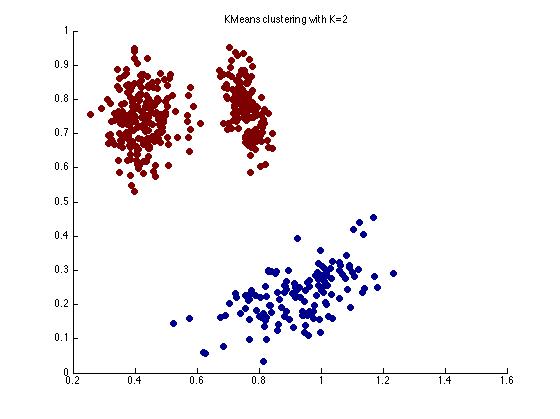
\includegraphics[width=0.75\textwidth]{../figures/k2.png}
  \caption{KMeans Clustering with K=2}
\end{figure}

\begin{figure}[h!]
  \centering
    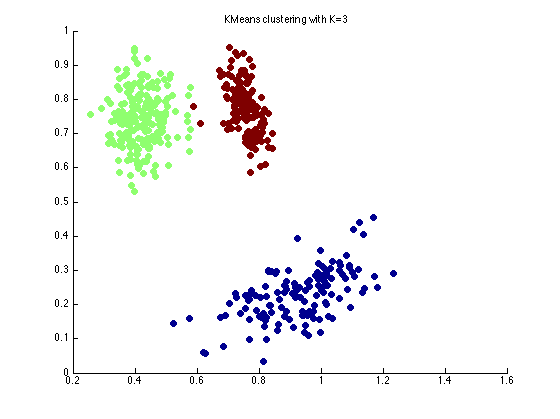
\includegraphics[width=0.75\textwidth]{../figures/k3.png}
  \caption{KMeans Clustering with K=3}
\end{figure}

\begin{figure}[h!]
  \centering
    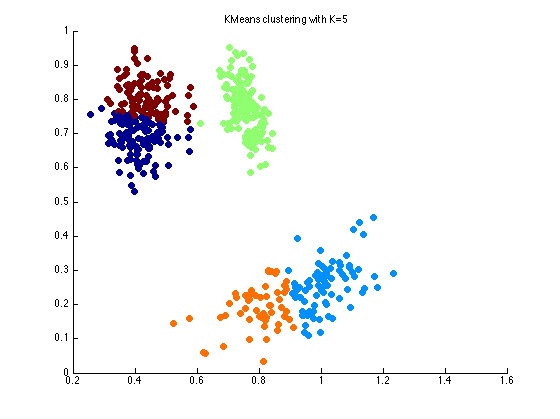
\includegraphics[width=0.8\textwidth]{../figures/k5.png}
  \caption{KMeans Clustering with K=5}
\end{figure}

\subsubsection{}
\begin{figure}[h!]
  \centering
    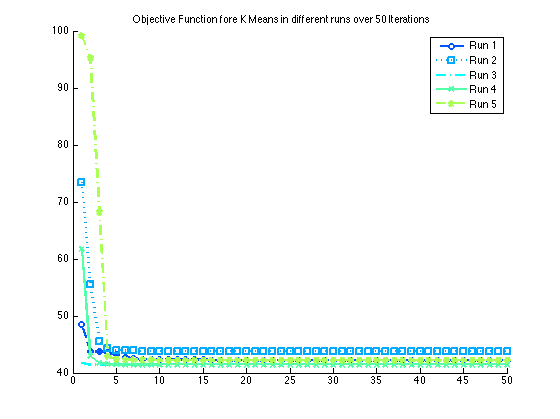
\includegraphics[width=0.8\textwidth]{../figures/fig5_1_b.png}
  \caption{Cost Function for KMeans for random initializations and K=4}
\end{figure}


\subsubsection{}
K means always converge because its objective function is the distance between points in the space. As there are only finite number of assignments for $\mu$ which is calculated from the given data points.\\\\
Though it may happen that, it may converge to global optimum rather than local optimum and in few cases may take exponential amount of time to converge. But the convergence is gauranteed.\\\\
In our data it can be seen that most of them converge within 5 iterations itself.

\subsection{}
\begin{figure}[h!]
  \centering
    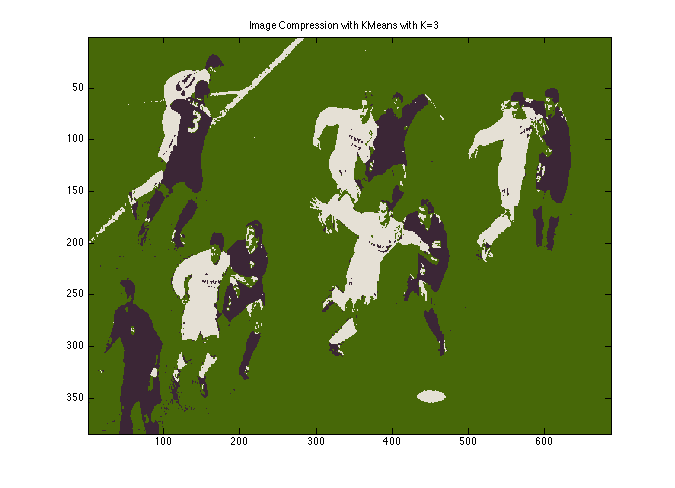
\includegraphics[width=0.9\textwidth]{../figures/football_k3.png}
  \caption{Reconstructed Image for K=3}
\end{figure}

\begin{figure}[h!]
  \centering
    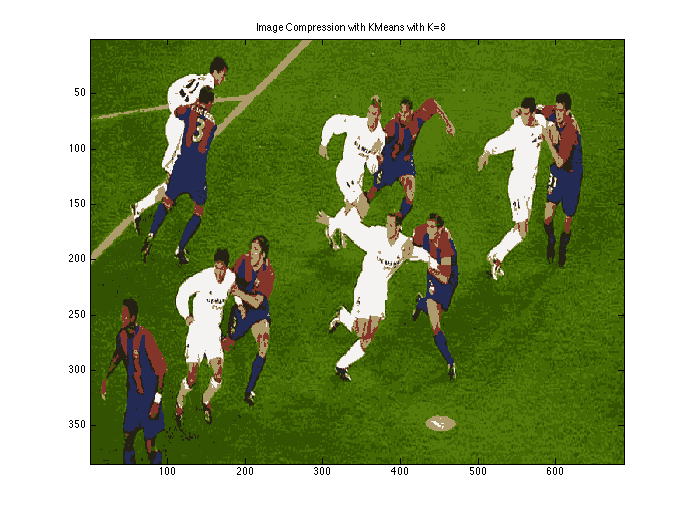
\includegraphics[width=0.9\textwidth]{../figures/football_k8.png}
  \caption{Reconstructed Image for K=8}
\end{figure}

\begin{figure}[h!]
  \centering
    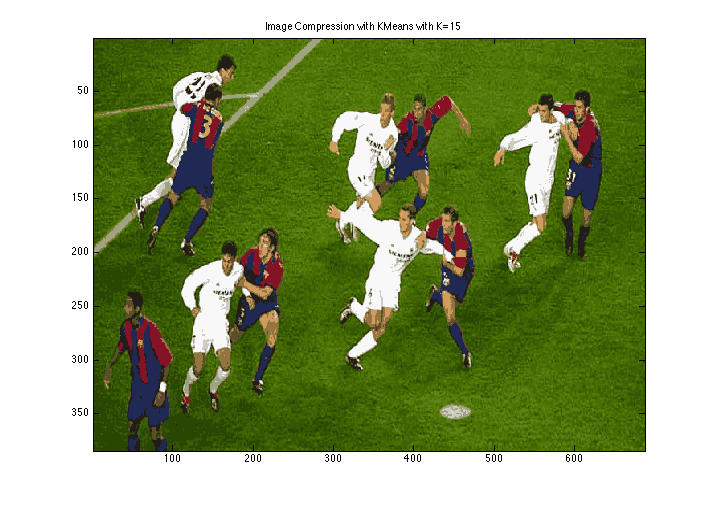
\includegraphics[width=0.9\textwidth]{../figures/football_k15.png}
  \caption{Reconstructed Image for K=15}
\end{figure}

\end{document}